\section{Flow Shops} \label{sec:7}
In many cases, each job has to undergo a series of operations. 
Often, these operations have to be done on all jobs in the same
order, implying that the jobs have to follow the same route.
The machines are then assumed to be set up in series and the environment 
is referred to as a flow shop. We saw an example of this in 
Example~\ref{exmp:1.3}; other real life examples are manufacturing and 
assembly facilities. 

We will mainly consider the makespan objective. The makespan objective is of 
considerable practical interest as its minimization is to a certain extent 
equivalent to the maximization of the utilization of the
machines. The models, however, tend to be of such complexity that makespan
results are already relatively hard to obtain. Total completion time and due
date related objectives tend to be even harder.

\subsection{Permutation Flow Shops} \label{subsec:7.1}
When searching for an optimal schedule for $(F_m~||~C_{\max})$, 
a natural question to ask is whether it suffices merely to determine 
a permutation in which the jobs traverse the entire system. 
It may be possible for one job to ``pass'' another while they are 
waiting in queue for a machine that is busy. This means that the 
machines might not be operating according to the ``first come first 
served'' principle, and that the sequence in which the jobs go through the 
machines may change from one machine to another. Changing the sequence of the 
jobs waiting in a queue between two machines may at times result in a smaller 
makespan. However, it can be shown that there always exists an optimal 
schedule without job sequence changes between the first two machines 
and the last two machines. This implies that there are optimal schedules for 
$(F_2~||~C_{\max})$ and $(F_3~||~C_{\max})$ that do not require 
sequence changes between machines. There are examples of flow shops with 
four machines in which the optimal schedule does require a job sequence 
change between the second and third machine. 

Finding an optimal schedule when sequence changes are allowed is significantly
harder than finding an optimal schedule when sequence changes are not
allowed. Flow shops that do not allow sequence changes between machines are
called {\bf permutation flow shops}. In these flow shops, the same sequence, 
or permutation, of jobs is maintained throughout. We denote this 
problem by $(F_m~|~\text{prmu}~|~C_{\max})$. Many results we will
look at concern permutation flow shops. 

Given a permutation schedule $j_1, \dots, j_n$ for a flow shop with $m$ 
machines, the completion time of a job $j_k$ at machine $i$ can be 
computed through a set of recursive equations. In particular, we have 
\begin{align*}
    C_{i,j_1} &= \sum_{\ell=1}^i p_{\ell,j_1}, && i = 1, \dots, m, \\ 
    C_{1,j_k} &= \sum_{\ell=1}^k p_{1,j_\ell}, && k = 1, \dots, n, \\ 
    C_{i,j_k} &= \max\{C_{i-1,j_k}, C_{i,j_{k-1}}\} + p_{i,j_k}, && i = 2, \dots, m,\; k = 2, \dots, n.
\end{align*}
Under the permutation schedule $j_1, \dots, j_n$, we can also compute the 
makespan by determining a {\bf critical path} in a directed graph corresponding 
to the schedule. For each operation, say the processing of job $j_k$ 
on machine $i$, there is a node $(i, j_k)$ with a weight equal to the 
processing time of job $j_k$ on machine $i$. Each node $(i, j_k)$ 
for $i = 1, \dots, m-1$ and $k = 1, \dots, n-1$ has edges going out to 
nodes $(i+1, j_k)$ and $(i, j_{k+1})$. Nodes corresponding to machine $m$ 
only have one outgoing edge, as do nodes corresponding to job $j_n$.
The node $(m, j_n)$ has no outgoing edges. The total weight of the 
maximum weight path from node $(1, j_1)$ to node $(m, j_n)$ is the 
makespan under the permutation schedule $j_1, \dots, j_n$. 
We illustrate this directed graph below. 

\begin{center}
    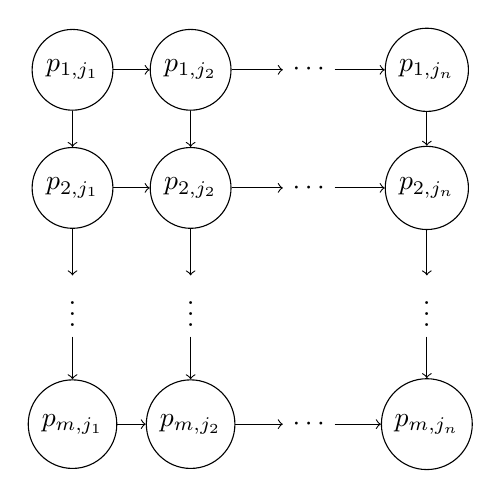
\begin{tikzpicture}              
        \node [circle, draw=black] (11) at (0, 8) {$p_{1,j_1}$};  
        \node [circle, draw=black] (12) at (1.5, 8) {$p_{1,j_2}$}; 
        \node (13) at (3, 8) {$\cdots$}; 
        \node [circle, draw=black] (14) at (4.5, 8) {$p_{1,j_n}$}; 
        
        \node [circle, draw=black] (21) at (0, 6.5) {$p_{2,j_1}$};
        \node [circle, draw=black] (22) at (1.5, 6.5) {$p_{2,j_2}$};
        \node (23) at (3, 6.5) {$\cdots$};
        \node [circle, draw=black] (24) at (4.5, 6.5) {$p_{2,j_n}$}; 
        
        \node (31) at (0, 5) {$\vdots$};
        \node (32) at (1.5, 5) {$\vdots$};
        \node (34) at (4.5, 5) {$\vdots$};

        \node [circle, draw=black] (41) at (0, 3.5) {$p_{m,j_1}$};
        \node [circle, draw=black] (42) at (1.5, 3.5) {$p_{m,j_2}$};
        \node (43) at (3, 3.5) {$\cdots$};
        \node [circle, draw=black] (44) at (4.5, 3.5) {$p_{m,j_n}$};
        
        \draw [->] (11) -- (12); \draw [->] (12) -- (13); \draw [->] (13) -- (14);
        \draw [->] (21) -- (22); \draw [->] (22) -- (23); \draw [->] (23) -- (24);
        \draw [->] (41) -- (42); \draw [->] (42) -- (43); \draw [->] (43) -- (44);
        \draw [->] (11) -- (21); \draw [->] (21) -- (31); \draw [->] (31) -- (41);
        \draw [->] (12) -- (22); \draw [->] (22) -- (32); \draw [->] (32) -- (42);
        \draw [->] (14) -- (24); \draw [->] (24) -- (34); \draw [->] (34) -- (44);
    \end{tikzpicture} 
\end{center}

\begin{exmp}{exmp:7.1}
    Consider $n = 5$ jobs on $m = 4$ machines with the processing times below. 
    \begin{align*}
        \begin{array}{c|ccccc}
            \text{Jobs} & j_1 & j_2 & j_3 & j_4 & j_5 \\ \hline 
            p_{1,j_k} & 5 & 5 & 3 & 6 & 3 \\ 
            p_{2,j_k} & 4 & 4 & 2 & 4 & 4 \\ 
            p_{3,j_k} & 4 & 4 & 3 & 4 & 1 \\ 
            p_{4,j_k} & 3 & 6 & 3 & 2 & 5             
        \end{array}
    \end{align*}
    Under the sequence $j_1, j_2, j_3, j_4, j_5$, the corresponding 
    graph and Gantt chart are given below. 
    In the top right corner of each node in the directed graph, we put the 
    completion time of that node. It follows that the makespan is 
    $C_{\max} = 34$, and it is determined by the two critical paths given in red.
    \begin{center}
        \begin{tikzpicture}[/pgfgantt/y unit chart=0.65cm] 
            \begin{ganttchart}[
                title/.style={draw=none},
                canvas/.append style={draw=none}, 
                bar top shift=0.1, bar height=0.6,
                y unit title=0.65cm,
                x unit=0.37cm
            ]{1}{40}
                \ganttbar{$M_1$}{1}{5} \ganttbar[inline]{5}{1}{5} \ganttbar[inline]{5}{6}{10} \ganttbar[inline]{3}{11}{13} \ganttbar[inline]{6}{14}{19} \ganttbar[inline]{3}{20}{22} \\ 
                \ganttbar{$M_2$}{6}{9} \ganttbar[inline]{4}{6}{9} \ganttbar[inline]{4}{11}{14} \ganttbar[inline]{2}{15}{16} \ganttbar[inline]{4}{20}{23} \ganttbar[inline]{4}{24}{27} \\ 
                \ganttbar{$M_3$}{10}{13} \ganttbar[inline]{4}{10}{13} \ganttbar[inline]{4}{15}{18} \ganttbar[inline]{3}{19}{21} \ganttbar[inline]{4}{24}{27} \ganttbar[inline]{1}{28}{28} \\ 
                \ganttbar{$M_4$}{14}{16} \ganttbar[inline]{3}{14}{16} \ganttbar[inline]{6}{19}{24} \ganttbar[inline]{3}{25}{27} \ganttbar[inline]{2}{28}{29} \ganttbar[inline]{5}{30}{34} \\ 
                \gantttitlelist{1,...,34}{1}
            \end{ganttchart}
        \end{tikzpicture}
        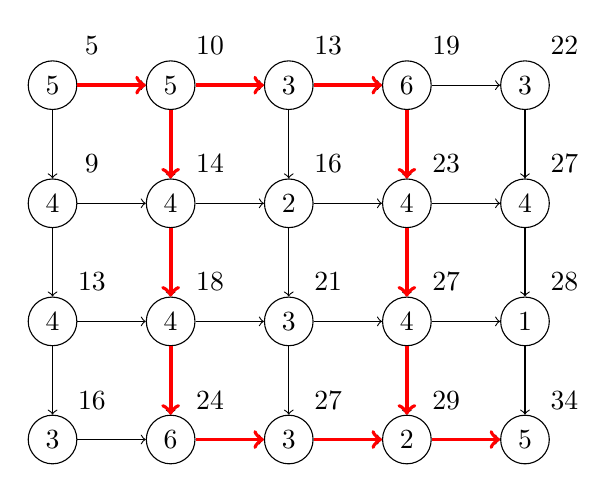
\begin{tikzpicture}              
            \node [circle, draw=black] (11) at (0, 8) {$5$};  
            \node [circle, draw=black] (12) at (1.5, 8) {$5$}; 
            \node [circle, draw=black] (13) at (3, 8) {$3$}; 
            \node [circle, draw=black] (14) at (4.5, 8) {$6$}; 
            \node [circle, draw=black] (15) at (6, 8) {$3$}; 
            
            \node [circle, draw=black] (21) at (0, 6.5) {$4$};
            \node [circle, draw=black] (22) at (1.5, 6.5) {$4$};
            \node [circle, draw=black] (23) at (3, 6.5) {$2$};
            \node [circle, draw=black] (24) at (4.5, 6.5) {$4$};
            \node [circle, draw=black] (25) at (6, 6.5) {$4$};
            
            \node [circle, draw=black] (31) at (0, 5) {$4$};
            \node [circle, draw=black] (32) at (1.5, 5) {$4$};
            \node [circle, draw=black] (33) at (3, 5) {$3$};
            \node [circle, draw=black] (34) at (4.5, 5) {$4$};
            \node [circle, draw=black] (35) at (6, 5) {$1$};
            
            \node [circle, draw=black] (41) at (0, 3.5) {$3$};
            \node [circle, draw=black] (42) at (1.5, 3.5) {$6$};
            \node [circle, draw=black] (43) at (3, 3.5) {$3$};
            \node [circle, draw=black] (44) at (4.5, 3.5) {$2$};
            \node [circle, draw=black] (45) at (6, 3.5) {$5$};
            
            \node (11') at (0.5, 8.5) {$5$};
            \node (12') at (2, 8.5) {$10$};
            \node (13') at (3.5, 8.5) {$13$};
            \node (14') at (5, 8.5) {$19$};
            \node (15') at (6.5, 8.5) {$22$};
            
            \node (21') at (0.5, 7) {$9$};
            \node (22') at (2, 7) {$14$};
            \node (23') at (3.5, 7) {$16$};
            \node (24') at (5, 7) {$23$};
            \node (25') at (6.5, 7) {$27$};
            
            \node (31') at (0.5, 5.5) {$13$};
            \node (32') at (2, 5.5) {$18$};
            \node (33') at (3.5, 5.5) {$21$};
            \node (34') at (5, 5.5) {$27$};
            \node (35') at (6.5, 5.5) {$28$};
            
            \node (41') at (0.5, 4) {$16$};
            \node (42') at (2, 4) {$24$};
            \node (43') at (3.5, 4) {$27$};
            \node (44') at (5, 4) {$29$};
            \node (45') at (6.5, 4) {$34$};
            
            \foreach \x in {1,...,4}
            { 
                \foreach \y in {1,...,4}
                {
                    \pgfmathtruncatemacro{\cur}{10*\x + \y}
                    \pgfmathtruncatemacro{\next}{\cur + 1}
                    \draw [->] (\cur) -- (\next); 
                }
            }
            
            \foreach \x in {1,...,3}
            { 
                \foreach \y in {1,...,5}
                {
                    \pgfmathtruncatemacro{\curvert}{10*\x + \y}
                    \pgfmathtruncatemacro{\nextvert}{\curvert + 10}
                    \draw [->] (\curvert) -- (\nextvert); 
                }
            }
            
            \draw[->, draw=red, line width=0.5mm] (11) -- (12);
            \draw[->, draw=red, line width=0.5mm] (12) -- (13);
            \draw[->, draw=red, line width=0.5mm] (13) -- (14);
            \draw[->, draw=red, line width=0.5mm] (12) -- (22);
            \draw[->, draw=red, line width=0.5mm] (22) -- (32);
            \draw[->, draw=red, line width=0.5mm] (32) -- (42);
            \draw[->, draw=red, line width=0.5mm] (14) -- (24);
            \draw[->, draw=red, line width=0.5mm] (24) -- (34);
            \draw[->, draw=red, line width=0.5mm] (34) -- (44);
            \draw[->, draw=red, line width=0.5mm] (42) -- (43);
            \draw[->, draw=red, line width=0.5mm] (43) -- (44);
            \draw[->, draw=red, line width=0.5mm] (44) -- (45);
        \end{tikzpicture} 
    \end{center}
\end{exmp}

\subsection{Johnson's Rule} \label{subsec:7.2}
We now consider the $(F_2~||~C_{\max})$ problem. Note that there 
is no permutation schedule restriction here, as we noted that 
$(F_2~||~C_{\max})$ has an optimal schedule that is a permutation schedule. 
There are two machines and $n$ jobs, with processing time $a_j = p_{1j}$ on 
machine $1$ and processing time $b_j = p_{2j}$ on machine $2$. This was one of 
the first problems to be analyzed in the early days of operations research 
and led to a classical paper in scheduling theory by S. M. Johnson. 
The rule that minimizes the makespan is commonly referred to as 
Johnson's rule. 

\begin{algo}[Johnson's rule]{algo:7.2}
    \begin{enumerate}[(1)]
        \item Set $i = 1$, $\ell = n$, and $\hat J = [n]$. 
        \item If $\hat J = \varnothing$, then stop. Otherwise, set 
        $\mu = \min\{a_j, b_j : j \in \hat J\}$. 
        \item \begin{enumerate}[(a)]
            \item If $\mu = a_j$, then place job $j$ in position $i$
            of the sequence. Increase $i$ by $1$ and delete $j$ from 
            $\hat J$. Go back to Step 2. 
            \item If $\mu = b_j$, then place job $j$ in position $\ell$
            of the sequence. Decrease $\ell$ by $1$ and delete $j$ from 
            $\hat J$. Go back to Step 2. 
        \end{enumerate} 
    \end{enumerate}
\end{algo}

\begin{exmp}{exmp:7.3}
    Consider the following $n = 5$ jobs on two machines. 
    \begin{align*}
        \begin{array}{c|ccccc}
            j & 1 & 2 & 3 & 4 & 5 \\ \hline 
            a_j & 5 & 2 & 3 & 6 & 3 \\ 
            b_j & 1 & 4 & 3 & 4 & 4
        \end{array}
    \end{align*}
    Then at iteration 1, we have $\mu = b_1 = 1$, so we put job $1$ 
    in position $5$. At iteration 2, we have $\mu = a_2 = 2$, so we put 
    job $2$ in position $1$. At iteration 3, we arbitrarily pick 
    $\mu = a_3 = 3$, so job $3$ goes in position $2$. At iteration 4, 
    we get $\mu = a_5 = 3$, so job $5$ goes in position $3$. Finally, job 
    $4$ goes in position $4$, so we obtain the final sequence 
    $2, 3, 5, 4, 1$. 
\end{exmp}

Note that Johnson's rule is equivalent to the following algorithm. 
Partition the jobs into two sets: $S_1$ contains all jobs $j$ with 
$a_j \leq b_j$, and $S_2$ contains all jobs $j$ with $a_j > b_j$. 
Place the jobs in $S_1$ first in SPT order, and the jobs in $S_2$ last 
in LPT order. In this sense, this is also called the SPT(1)-LPT(2) rule. 

Let us now show that Johnson's rule is indeed optimal for 
$(F_2~||~C_{\max})$. We first prove a key lemma. 

\begin{lemma}{lemma:7.4}
    \begin{enumerate}[(1)]
        \item If $\mu = a_j = \min\{a_\ell, b_\ell : \ell \in [n]\}$ in the 
        first iteration of Johnson's rule, then there is an optimal schedule 
        that places job $j$ first. 
        \item If $\mu = b_j = \min\{a_\ell, b_\ell : \ell \in [n]\}$ in the 
        first iteration of Johnson's rule, then there is an optimal schedule 
        that places job $j$ last. 
    \end{enumerate}
\end{lemma}
\begin{pf}
    We will only prove (1), as the proof of (2) is analogous. 
    Suppose that we have an optimal schedule $S^*$ that does not start with 
    job $j$. Then there must be a job $\ell$ immediately preceding $j$ in 
    $S$. Let $t_\ell^1$ denote the starting time of $\ell$ on machine $1$, 
    and let $t_\ell^2$ denote the starting time of $\ell$ on machine $2$. 
    We interchange jobs $j$ and $\ell$ to get a new schedule $S'$. 

    We claim that $C'_\ell \leq C_j$, where $C'_\ell$ is the completion time 
    of job $\ell$ in $S'$ and $C_j$ is the completion time of job $j$ in $S$. 
    Observe that in the directed graph representation under $S$, 
    there are three possible paths we could take, illustrated below. 
    \begin{center}
        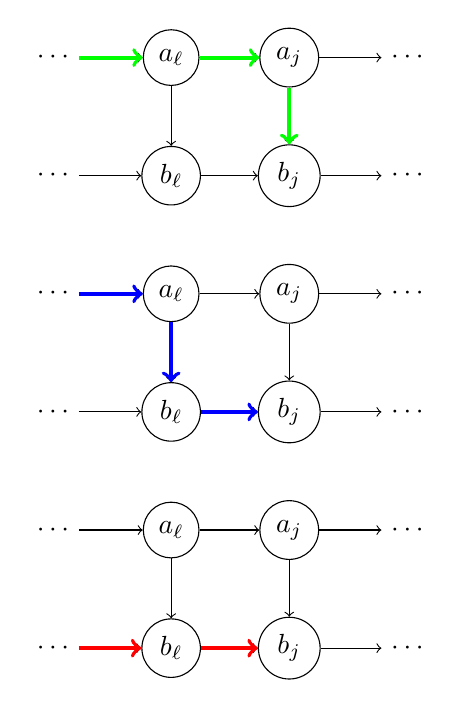
\begin{tikzpicture}              
            \node (111) at (0, 8) {$\cdots$};  
            \node [circle, draw=black] (112) at (1.5, 8) {$a_\ell$}; 
            \node [circle, draw=black] (113) at (3, 8) {$a_j$}; 
            \node (114) at (4.5, 8) {$\cdots$}; 
            
            \node (121) at (0, 6.5) {$\cdots$};  
            \node [circle, draw=black] (122) at (1.5, 6.5) {$b_\ell$}; 
            \node [circle, draw=black] (123) at (3, 6.5) {$b_j$}; 
            \node (124) at (4.5, 6.5) {$\cdots$}; 
            
            \node (211) at (0, 5) {$\cdots$};  
            \node [circle, draw=black] (212) at (1.5, 5) {$a_\ell$}; 
            \node [circle, draw=black] (213) at (3, 5) {$a_j$}; 
            \node (214) at (4.5, 5) {$\cdots$}; 
            
            \node (221) at (0, 3.5) {$\cdots$};  
            \node [circle, draw=black] (222) at (1.5, 3.5) {$b_\ell$}; 
            \node [circle, draw=black] (223) at (3, 3.5) {$b_j$}; 
            \node (224) at (4.5, 3.5) {$\cdots$}; 
            
            \node (311) at (0, 2) {$\cdots$};  
            \node [circle, draw=black] (312) at (1.5, 2) {$a_\ell$}; 
            \node [circle, draw=black] (313) at (3, 2) {$a_j$}; 
            \node (314) at (4.5, 2) {$\cdots$}; 
            
            \node (321) at (0, 0.5) {$\cdots$};  
            \node [circle, draw=black] (322) at (1.5, 0.5) {$b_\ell$}; 
            \node [circle, draw=black] (323) at (3, 0.5) {$b_j$}; 
            \node (324) at (4.5, 0.5) {$\cdots$}; 

            \draw [->] (111) -- (112); \draw [->] (112) -- (113); \draw [->] (113) -- (114); 
            \draw [->] (121) -- (122); \draw [->] (122) -- (123); \draw [->] (123) -- (124);
            \draw [->] (112) -- (122); \draw [->] (113) -- (123); 

            \draw [->] (211) -- (212); \draw [->] (212) -- (213); \draw [->] (213) -- (214); 
            \draw [->] (221) -- (222); \draw [->] (222) -- (223); \draw [->] (223) -- (224);
            \draw [->] (212) -- (222); \draw [->] (213) -- (223); 

            \draw [->] (311) -- (312); \draw [->] (312) -- (313); \draw [->] (313) -- (314); 
            \draw [->] (321) -- (322); \draw [->] (322) -- (323); \draw [->] (323) -- (324);
            \draw [->] (312) -- (322); \draw [->] (313) -- (323); 
            
            \draw[->, draw=green, line width=0.5mm] (111) -- (112);
            \draw[->, draw=green, line width=0.5mm] (112) -- (113);
            \draw[->, draw=green, line width=0.5mm] (113) -- (123);

            \draw[->, draw=blue, line width=0.5mm] (211) -- (212);
            \draw[->, draw=blue, line width=0.5mm] (212) -- (222);
            \draw[->, draw=blue, line width=0.5mm] (222) -- (223);

            \draw[->, draw=red, line width=0.5mm] (321) -- (322);
            \draw[->, draw=red, line width=0.5mm] (322) -- (323);
        \end{tikzpicture} 
    \end{center}
    Note that the green path is dominated by the blue path because 
    $a_j \leq b_\ell$ by assumption. This shows that 
    \[ C_j = \max\{t_\ell^2 + b_\ell + b_j, t_\ell^1 + a_\ell + b_\ell + b_j\}. \] 
    Constructing a similar diagram for $S'$ gives us 
    \[ C'_\ell = \max\{t_\ell^1 + a_j + a_\ell + b_\ell, 
    t_\ell^1 + a_j + b_j + b_\ell, 
    t_\ell^2 + b_j + b_\ell\}. \] 
    Noting that $a_j = \min\{a_j, b_j : j \in [n]\}$, it is easy to 
    check that $C_j \geq C'_\ell$ by comparing the terms above. 
    This means that $S'$ is also an optimal schedule which has job $j$ 
    before job $\ell$. We can continue to interchange jobs and 
    repeat our argument until job $j$ is first. 
\end{pf}

\begin{theo}{theo:7.5}
    Johnson's rule gives an optimal schedule for $(F_2~||~C_{\max})$. 
\end{theo}
\begin{pf}
    We give a sketch of the proof. We proceed by induction on the number 
    of iterations. The earlier iterations would have constructed a 
    partial schedule. Apply Lemma~\ref{lemma:7.4} to the set of jobs 
    that remain to be scheduled after $i-1$ iterations. Note that 
    Lemma~\ref{lemma:7.4} only sees the two jobs $j$ minimizing the 
    value of $\mu$ and the job $\ell$ immediately preceding job $j$; 
    it ``ignores'' all other jobs. 
\end{pf}

As one might imagine, a schedule obtained from Johnson's rule is 
by no means the only schedule that is optimal for $(F_2~||~C_{\max})$. 
The class of optimal schedules appears to be hard to characterize and 
data dependent. 

\subsection{Mixed Integer Program Formulation for Permutation Schedules} \label{subsec:7.3}
Unfortunately, the schedule structure from Johnson's rule cannot be 
generalized to characterize optimal schedules for flow shops with 
more than two machines. Indeed, it turns out that even the three machine case 
is strongly $\NP$-hard. 

\begin{theo}{theo:7.6}
    The problem $(F_3~||~C_{\max})$ is strongly $\NP$-hard. 
\end{theo}
\begin{pf}
    We prove this via a reduction from \textsc{$3$-Partition}. Given 
    $a_1, \dots, a_{3t}, b \in \Z^+$ under the usual assumptions, 
    let the number of jobs be $n = 4t+1$, and let the processing times be 
    \begin{align*}
        p_{10} &= 0, & p_{20} &= b, & p_{30} &= 2b, \\ 
        p_{1j} &= 2b, & p_{2j} &= b, & p_{3j} &= 2b, & j &= 1, \dots, t-1, \\ 
        p_{1t} &= 2b, & p_{2t} &= b, & p_{3t} &= 3b, \\ 
        p_{1,t+j} &= 0, & p_{2,t+j} &= a_j, & p_{3,t+j} &= 0, & j &= 1, \dots, 3t. 
    \end{align*}
    Let $z = (2t+1)b$. A makespan of value $z$ can be obtained if the first 
    $t+1$ jobs are scheduled according to the sequence $0, 1, \dots, t$. 
    These $t+1$ jobs then form a framework, leaving $t$ gaps on machine $2$. 
    Then jobs $t+1, \dots, 4t$ have to be partitioned into $t$ sets of three 
    jobs each, and these $t$ sets have to be scheduled between the first 
    $t+1$ jobs. Thus, a makespan of $z$ can be obtained if and only if 
    the \textsc{$3$-Partition} instance has a solution. 
\end{pf}

The problem $(F_m~|~\text{prmu}~|~C_{\max})$ can be formulated 
as a mixed integer program (MIP). Note that the fact that the problem 
can be formulated in this way does not imply that the problem is 
$\NP$-hard. It could be that the MIP has a special structure that 
allows for a polynomial time algorithm, such as the one we saw 
for $(R_m~||~\sum C_j)$ in Section~\ref{subsec:6.4}. However, 
Theorem~\ref{theo:7.6} shows that this is not the case. 

We first define some variables that we need.
\begin{itemize}
    \item Let $x_{jk}$ be a binary variable equal to $1$ if job $j$ is the 
    $k$-th job in the sequence, and $0$ otherwise. 
    \item The auxiliary variable $I_{ik}$ denotes the idle time on machine $i$
    between the processing of the jobs in the $k$-th and $(k+1)$-th positions. 
    \item The auxiliary variable $W_{ik}$ denotes the waiting time of the 
    job in the $k$-th position between machines $i$ and $i+1$. 
\end{itemize} 
Naturally, there is a strong relationship between the variables $W_{ik}$ and 
the variables $I_{ik}$. For example, if $I_{ik} > 0$, then 
$W_{i-1,k+1} = 0$. Formally, this relationship can be established by 
considering the difference between the time the job in the $(k+1)$-th 
position starts on machine $i+1$ and the time the job in the $k$-th position 
completes its processing on machine $i$. If $\Delta_{ik}$ denotes this 
difference and $p_{i(k)}$ is the processing time of the job in the 
$k$-th position on machine $i$, then 
\[ \Delta_{ik} = I_{ik} + p_{i(k+1)} + W_{i,k+1} = W_{ik} + p_{i+1(k)} 
+ I_{i+1,k}. \] 
Note that minimizing the makespan is equivalent to minimizing the 
total idle time on the last machine, namely machine $m$. This idle 
time is equal to 
\[ \sum_{i=1}^{m-1} p_{i(1)} + \sum_{j=1}^{n-1} I_{mj}, \] 
which is the idle time that must occur before the job in the first position 
reaches the last machine and the sum of the idle times between the jobs 
on the last machine. Moreover, we have the identity
\[ p_{i(k)} = \sum_{j=1}^n x_{jk} p_{ij}. \] 
Putting everything together, we can now formulate the MIP as follows: 
\begin{align*}
    \min\quad & \sum_{i=1}^{m-1} \sum_{j=1}^n x_{j1} p_{ij} + \sum_{j=1}^{n-1} I_{mj} \\ 
    \text{s.t.}\quad & \sum_{j=1}^n x_{jk} = 1, && k \in [n] \\ 
    & \sum_{k=1}^n x_{jk} = 1, && j \in [n] \\ 
    & I_{ik} + \sum_{j=1}^n x_{j,k+1} p_{ij} + W_{i,k+1} - W_{ik} 
    - \sum_{j=1}^n x_{jk} p_{i+1,j} - I_{i+1,k} = 0, && k \in [n-1],\; i \in [m-1] \\
    & W_{i1} = 0, && i \in [m-1] \\
    & I_{1k} = 0, && k \in [n-1].
\end{align*}
The first set of constraints specifies that exactly one job has to be assigned to
position $k$ for any $k$. The second set of constraints specifies that job $j$ has to be
assigned to exactly one position. The third set of constraints relate the decision
variables $x_{jk}$ to the physical constraints. These physical constraints enforce the
necessary relationships between the idle time variables and the waiting time
variables. Thus, the problem of minimizing the makespan in an $m$ machine
permutation flow shop is formulated as an MIP. The only integer variables
are the binary decision variables $x_{jk}$. The idle time and waiting time
variables are non-negative continuous variables.